\section*{Study design and data}
\begin{figure*}[t]\centering
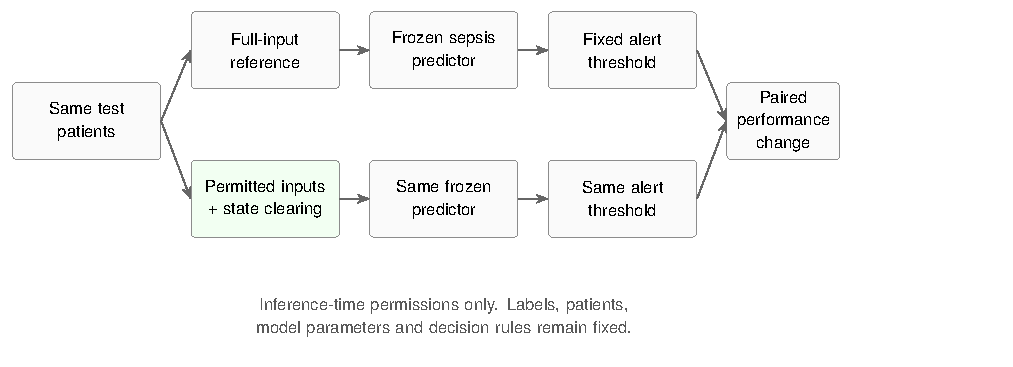
\includegraphics[width=\linewidth]{figs/paired_design.pdf}
\caption{The consent comparison changes inference-time permissions while holding patients, labels, fitted model parameters and alert thresholds fixed. The restricted branch clears denied features and, after revocation, recurrent state. Paired effects measure the behavior of these fixed predictors; they are not effects of withholding treatment or retraining on a different cohort.}
\end{figure*}


The benchmark compares full-input AI with consent-constrained AI on the same held-out patients. We define the constrained system by the inputs it may process and the derived state it must clear. The experiment is designed to measure how that intervention changes performance, rather than assume that consent has either no cost or an unavoidable fixed cost. Sepsis provides a concrete, public evaluation setting; generalization to other diseases is not established by this study.

We use version 1.0.0 of the public PhysioNet/CinC 2019 release \citep{physionet,reyna2020}. Hospital A contributes 20,336 patient files and 790,215 hourly records; hospital B contributes 20,000 files and 761,995 records. Together they contain 1,552,210 rows. Each record contains 40 input variables: eight vital signs, 26 laboratory variables and six demographic or administrative variables, plus the supplied SepsisLabel. No video, skeleton or credentialed dataset contributes to the revised primary analysis.

The cohort is defined by the full public-file manifest, not by selecting a favorable subset. Downloads are checked against the published object ETag, and a SHA256 digest is recorded for each local file. Patient IDs, site membership, row boundaries and split assignments are retained in the released provenance. The public source is already de-identified; the study does not link records to external identities or collect new patient information. Dataset terms and evaluator licensing accompany the release.

\begin{table}[t]
\centering\small
\caption{Public cohort and incident eligibility. ``Positive'' means at least one positive label. The two exclusion categories concern the strict incident endpoint; all patients remain in workload calculations.}

\begin{tabular}{lrr}\toprule
Quantity & Hospital A & Hospital B\\\midrule
Patients & 20,336 & 20,000\\
Hourly records & 790,215 & 761,995\\
Label-positive patients & 1,790 & 1,142\\
Initial-positive patients & 203 & 223\\
Onset at/after observed end & 2 & 13\\
Eligible incident patients & 1,585 & 906\\\bottomrule
\end{tabular}
\end{table}

The supplied label becomes positive six hours before inferred sepsis onset. Let $a_i$ be the index of patient $i$'s first positive label and set $o_i=a_i+6$. We use zero-based hourly indices. The strict warning window is $[a_i,o_i)$, containing the six observations immediately before inferred onset. The label is not shifted a second time.

A patient enters the conditional incident-risk denominator when $a_i>0$ and $o_i<T_i$, where $T_i$ is the number of observed rows. Initial-positive patients have no observed pre-window prefix, and patients whose inferred onset is at or beyond the observed end do not meet this complete-window definition. The cohort table reports these exclusions. This retrospective convention is stricter than simply asking whether a positive label ever occurs.

For workload, positive patients are monitored through $\min(o_i,T_i)$ and patients without a positive label through $T_i$. All patients, including those excluded from incident risk, remain in the workload denominator. The stopping time depends on the retrospective label, which would not be known to a deployed model. It therefore defines a benchmark accounting interval, not a prospective operational stopping mechanism. Full-stay challenge utility is computed separately. A later deployment study would need an observable endpoint, such as discharge or an independently recorded clinical decision, and would have to reevaluate workload under that endpoint.

For each seed in $\{11,29,47\}$, a seeded permutation of hospital A assigns 55\% to training, 15\% to validation, 15\% to calibration and 15\% to testing. Integer cut points produce 11,184 training, 3,051 validation, 3,050 calibration and 3,051 test patients. Hospital B is independently permuted into 5,000 local-calibration and 15,000 external-test patients. No B labels train the clinical predictor.

Every observation from a patient stays in one partition within a seed. Hyperparameters and candidate thresholds use training and validation only. Calibration is reserved for risk/workload certification; test data evaluate the frozen result. The three seed-specific test sets overlap, so the analysis reports seed variability descriptively rather than treating the runs as three independent clinical cohorts. Splitting is not stratified on the outcome; the positive calibration counts are reported explicitly.

At hour $t$, each of the 40 raw variables contributes its most recent observed value up to $t$. For the 34 physiological variables, we additionally calculate the expanding mean of observed values and the cumulative observation count. The feature vector therefore has $40+34+34=108$ entries. If $x_{itv}$ is variable $v$ and $m_{itv}$ indicates observation, the summaries are
\begin{align*}
 c_{itv}&=\sum_{u\le t}m_{iuv},\qquad
 \bar x_{itv}=\frac{\sum_{u\le t}m_{iuv}x_{iuv}}{c_{itv}},\\
 x^{\rm last}_{itv}&=x_{iu^*v},\quad
 u^*=\max\{u\le t:m_{iuv}=1\}.
\end{align*}
The mean and last value remain missing until an observation exists; the count is initially zero. SepsisLabel is excluded from the input. Forward filling and expanding summaries use only the current prefix. The code does not interpolate backward from a later measurement. Tests perturb future observations and verify that earlier feature values do not change.

Observation counts intentionally retain information about the measurement process. This can improve prediction but also makes consent interventions consequential: masking a value while retaining its historical count would leave a prohibited information path. Missingness-aware clinical models motivate treating the observation process explicitly \citep{che2018}; our count representation remains simpler than a dedicated missingness-decay architecture.

\section*{Prediction models and training}

All models predict the hourly supplied label using the same causal representation. Training loss and the primary discrimination evaluation omit rows from inferred onset onward. For a positive patient, the final included row is $\min(o_i,T_i)-1$; all observed rows of a label-negative patient are eligible. This prevents long post-onset stays from dominating the primary comparison. It does not remove the six pre-onset positive labels that define the prediction target.

The linear baseline imputes missing features with training-set means, retains initially empty feature columns, and applies training-set standardization. It fits an L2-regularized logistic model
\begin{equation*}
 s_{it}=\sigma(\beta^\top z_{it}+b),
\end{equation*}
where $z_{it}$ is the transformed feature vector. Four candidates combine inverse regularization $C\in\{0.1,1\}$ with either unweighted or class-balanced loss. The iteration limit is 350 and the random state follows the split seed. The selected model maximizes hourly validation average precision. This is a tuned linear baseline; it is not the fixed-$C$ predictor used in the archived initial study.

The nonlinear tabular baseline uses histogram gradient boosting, building an additive tree score under binary classification loss \citep{friedman2001}. Training-only variance screening removes constant and entirely missing columns; remaining missing values are handled by the estimator. The screening is necessary for the recorded implementation and uses no validation, calibration or test information.

The three candidates are $(15,1,\mathrm{unweighted})$, $(31,5,\mathrm{unweighted})$ and $(31,5,\mathrm{balanced})$, where the entries are maximum leaf count, L2 regularization and class weighting. Every candidate uses 120 boosting iterations, learning rate 0.08 and disabled automatic early stopping. Validation average precision chooses the candidate. The implementation uses scikit-learn \citep{sklearn}; the locked software version and exact parameter dictionaries are released. This small grid tests a stronger nonlinear predictor without claiming exhaustive hyperparameter optimization.

The sequence baseline has one unidirectional GRU layer \citep{cho2014} and a linear logit head at each hour:
\begin{equation*}
 h_{it}=\mathrm{GRU}(z_{it},h_{i,t-1}),\qquad
 s_{it}=\sigma(w^\top h_{it}+b).
\end{equation*}
Patient sequences are padded within batches and packed by their true lengths. Padding contributes no loss. The recurrent state is reset between patients. Although complete observed sequences can be passed through the forward computation, post-onset training positions are masked out of the loss; unidirectionality prevents later observations from influencing earlier outputs.

Training-set means and standard deviations normalize the 108 features. Empty or near-constant scales are replaced by one; normalized missing entries become zero and all normalized values are clipped to $[-10,10]$. Candidate hidden sizes are 32 and 64. Each candidate receives six epochs with Adam \citep{adam}, learning rate 0.001, batch size 64 and gradient-norm clipping at one. Training patients are reshuffled each epoch using the split seed.

The positive-weighted binary cross-entropy is
\begin{equation*}
 \mathcal L=-\frac{1}{|\mathcal I|}\sum_{(i,t)\in\mathcal I}
 \left[\omega y_{it}\log s_{it}+(1-y_{it})\log(1-s_{it})\right],
\end{equation*}
where $\mathcal I$ contains valid pre-onset training positions and $\omega=\min\{20,(1-\bar y)/\bar y\}$ uses the training prevalence. The implementation averages this loss over valid positions in each batch. Every epoch is evaluated on validation average precision; the best hidden-size/epoch pair is saved. There is no calibration-set early stopping, test-set model selection or bidirectional recurrence.

For all three model families, validation average precision is the sole model-selection criterion. AUROC is logged for the tabular candidates as a diagnostic. The selected estimators are frozen before calibration and before any consent or queue stress test. Prediction arrays preserve patient order and row boundaries for validation, A calibration, B calibration and both test sites. This allows later policy audits to reuse scores without retraining.

The search budgets differ by family: four logistic fits, three boosting fits and two six-epoch GRU trajectories per seed. They are appropriate for comparing these implementations, but they do not establish an architecture-level ranking under equal compute or equal tuning effort. We report both the settings and the selection rule so that a stronger model search can extend the study without changing its endpoints.
